\documentclass{article}
\usepackage{graphicx}
\usepackage[margin=1.5cm]{geometry}
\usepackage{amsmath}

\begin{document}
\twocolumn

\title{Wednesday warm-up: Kinematics, II and III}
\author{Prof. Jordan C. Hanson}

\maketitle

\begin{figure}
\centering
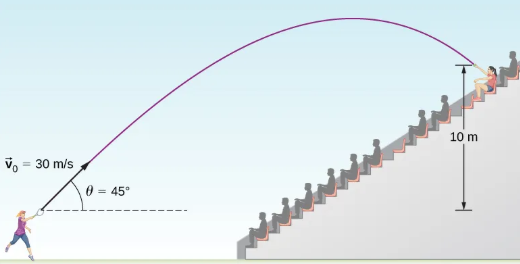
\includegraphics[width=0.45\textwidth]{figures/tennis.png}
\caption{\label{fig:1} A tennis player hits a ball into the stands.}
\end{figure}

\begin{figure}
\centering
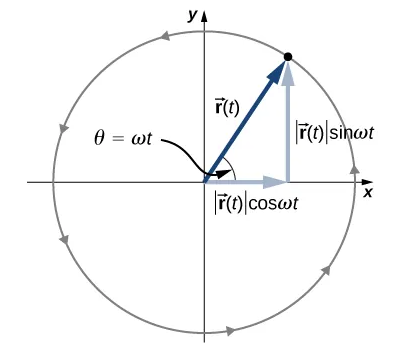
\includegraphics[width=0.3\textwidth]{figures/circular.png}
\caption{\label{fig:2} A diagram for uniform circular motion.}
\end{figure}

\section{Memory Bank}

\begin{enumerate}
\item $g = 9.81$ m s$^{-2}$
\item $v_x(t) = a_x t + v_{i,x}$
\item $v_y(t) = a_y t + v_{i,y}$
\item $x(t) = \frac{1}{2}a_x t^2 + v_{i,x} t + x_{i}$
\item $y(t) = \frac{1}{2}a_y t^2 + v_{i,y} t + x_{i}$
\item $v_f^2 = v_i^2 + 2a\Delta y$
\item $\vec{r}(t) = r \cos(\omega t) \hat{i} + r \sin(\omega t) \hat{j}$
\end{enumerate}

\section{Kinematics II}

\begin{enumerate}
\item After winning a match, a tennis player hits the ball into the stands at 30 m/s and at an angle 45 degrees above the horizontal (Fig. \ref{fig:1}).  The ball is caught by a spectator 10 m above the point where the ball was hit. (a) What is the horizontal component of the initial velocity?  (b) What is the vertical component of the initial velocity? \\ \vspace{1cm}
\item (a) Calculate the time it takes the tennis ball to reach the spectator. (b) What are the magnitude and direction of the ball's velocity at impact? \\ \vspace{4cm}
\item Consider Fig. \ref{fig:2}.  The angle $\theta(t) = \omega t$ describes the position of a system circling the origin at constant speed\footnote{The factor $\omega$ is the \textit{angular velocity}, in radians per second.}.  Show that
\begin{equation}
\vec{r}(t) = r \cos(\omega t) \hat{i} + r \sin(\omega t) \hat{j}
\end{equation} \vspace{2cm}
\item Show that the acceleration is $\vec{a} = -\omega^2 \vec{r}$.  Is the magnitude of the acceleration constant, or does it depend on time?
\end{enumerate}

\end{document}
